% ~~~ [ Code Coverage ] ~~~~~~~~~~~~~~~~~~~~~~~~~~~~~~~~~~~~~~~~~~~~~~~~~~~~~~~~

\subsubsection{Code Coverage}

\textbf{NOTE}: \textit{The following section is under construction :)}

The code coverage is a measurement of how much of the code is exercised by the test cases.

% As stated by Rob Pike, \textit{``Go was designed with tools in mind.''} \cite{go_cover}

The Go project takes an interesting approach to tracking code coverage. Instead of generating platform-dependent assembly which tracks the execution of various branches, Go exploits its support for source code analysis and manipulation to inject unique tracking statements on each line of the original source code \cite{go_cover}.

While developing a lexer for the LLVM IR assembly language the intention was to strive for a 100\% code coverage of any code related to lexing and not related to input output errors (e.g. ``file not found'' errors). As illustrated in figure \ref{fig:lexer_code_coverage}. The rigid testing made it possible to locate and correct a number of faulty assumptions in the lexing logic.

\begin{figure}[htbp]
	\begin{center}
		\begin{verbatim}
$ go test -coverprofile=lexer.out github.com/llir/llvm/asm/lexer
$ go tool cover -func=lexer.out
llvm/asm/lexer/lexer.go:36:    ParseFile      80.0%
llvm/asm/lexer/lexer.go:118:   emit           100.0%
llvm/asm/lexer/lexer.go:139:   next           100.0%
llvm/asm/lexer/lexer.go:158:   accept         100.0%
llvm/asm/lexer/state.go:38:    lexToken       100.0%
llvm/asm/lexer/state.go:131:   lexComment     100.0%
…
llvm/asm/lexer/state.go:364:   lexQuote       100.0%
llvm/asm/lexer/state.go:585:   unescape       100.0%
total:                         (statements)   97.5%
		\end{verbatim}
		\caption{A summary of the code coverage for a selection of the LLVM IR lexer functions, as visualized by the \texttt{cover} tool.}
		\label{fig:lexer_code_coverage}
	\end{center}
\end{figure}

The use of code coverage heat maps, which track how often statements are exercised by the test cases, were invaluable when stress testing the subgraph isomorphism search algorithm, and they were able to identify several tricky corner cases. foo figure \ref{fig:iso_heat_map}

\begin{figure}[htbp]
	\begin{center}
		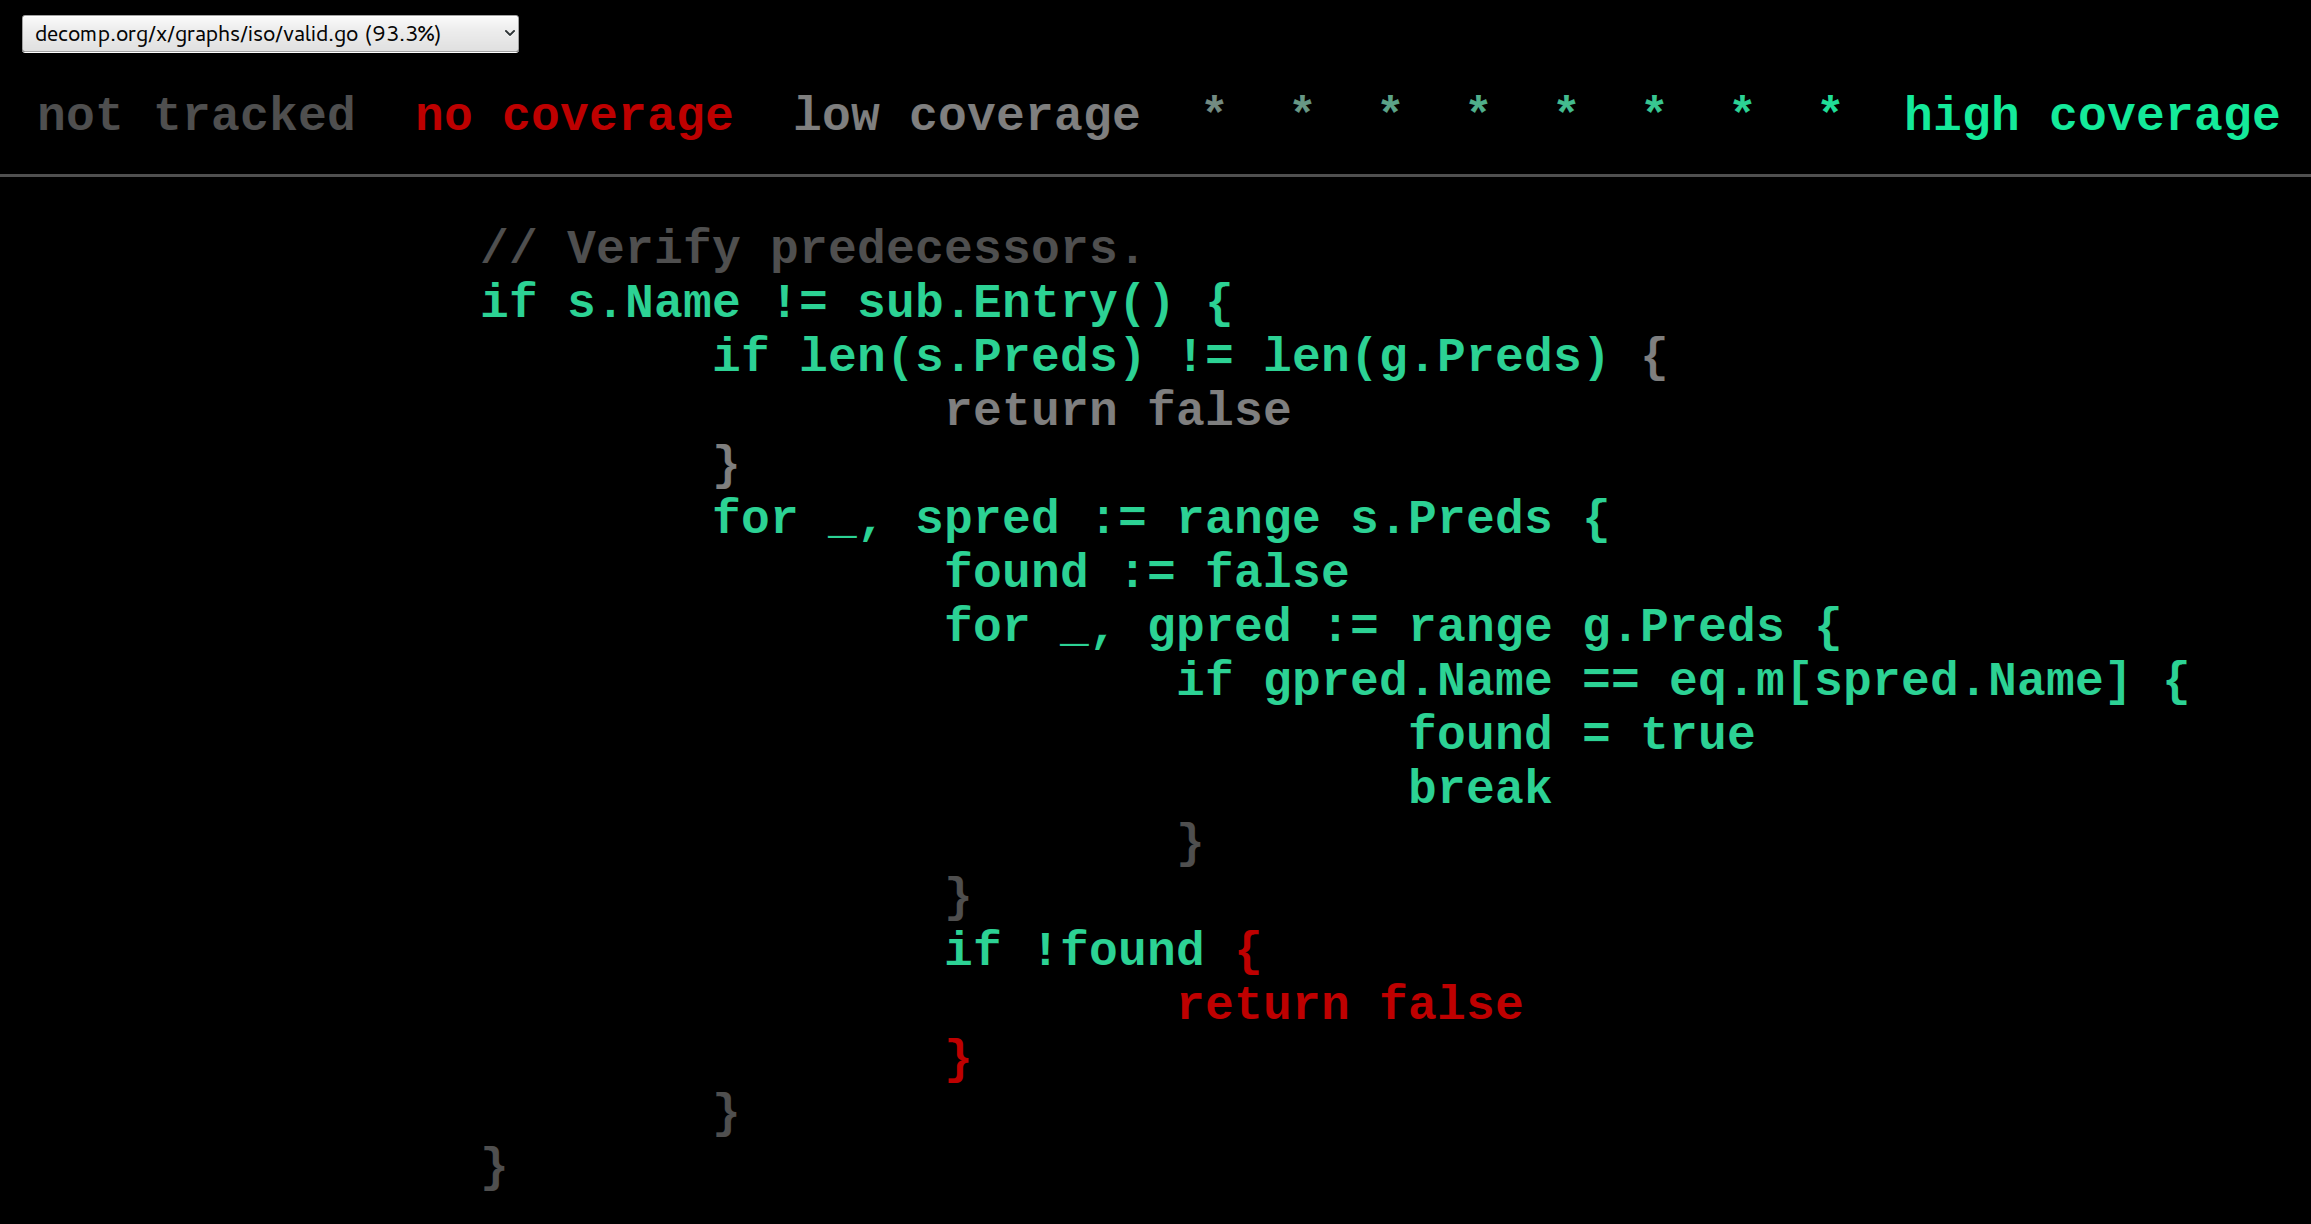
\includegraphics[width=\textwidth]{inc/8_ver/iso_heat_map.png}
		% TODO: Fix caption text.
		\caption{Extract from the code coverage of the subgraph isomorphism search algorithm, represented as a heat map where red indicates that a statement was never visited and the intensity of green indicates the number of times a statement was visited. where bright green represents a statements that has been visited several times, faint green a statement only visited a few times, and red a statement that has never been visited.}
		\label{fig:iso_heat_map}
	\end{center}
\end{figure}

foo
